\chapter{Natural Language Processing (NLP)}
Il \textbf{Natural Language Processing} (NLP) si occupa di studiare il linguaggio
naturale introducendo la semantica e le relazioni tra le parole. Oltre a questo,
si occupa di analizzare il testo, capire il contesto ed estrarre varie informazioni,
partendo dai topic fino ad arrivare alle emozioni.

In NLP la parte fondamentale è trovare una rappresentazione delle parole. Questo
non è una cosa banale in quanto:
\begin{itemize}
      \item Ci serve un contesto per rappresentare il testo in analisi.
      \item Ci può essere del rumore nei dati (dati errati o non fedeli).
      \item Può essere presente dell'ambiguità nelle frasi, per esempio abbiamo
            modi di dire. Questo viene risolto in diversi modi, ad esempio
            effettuando l'analisi sintattici, part-of-speech tagging, etc.
      \item Ambiguità sintattica, la quale viene risolta attraverso part-tree-disambiguation
\end{itemize}
I problemi legati all'\textbf{ambiguità morfo-sintattica} sono molto importanti
in questo campo, e sono studiati in modo approfondito. Per la loro risoluzione
esistono diverse tecniche che sono state sviluppate nel tempo e implementate in
librerie. Alcune di queste, forniscono sistemi per risolvere le ambiguità nelle
frasi, i quali si basano sulla costruzione di diversi alberi di parsing e
restituiscono l'albero della frase più probabile.

Tra le varie tipologie di ambiguità che possiamo incontrare distinguiamo due
tipologie:
\begin{itemize}
      \item \textbf{Ambiguità sintattica}: in una frase sono presenti più alberi
            di parsing. Questo viene studiato attraverso la \textbf{parse-tree-disambiguation}.
      \item \textbf{Ambiguità emozionale}: in una frase sono espresse emozioni
            contrastanti. Questo viene studiato attraverso la \textbf{sentiment analysis}.
      \item \textbf{Ambiguità semantica}: in una frase sono presenti parole che
            possono avere più significati. Questo viene studiato attraverso la
            \textbf{named-entity recognition} e in seguito il \textbf{named-entity
                  linking}.
\end{itemize}
\section{Sentiment analysis}
\begin{definizione}[\textbf{Text Analytics}]
      La \textbf{text analytics} è una tecnica che permette di estrarre informazioni
      dal linguaggio naturale per identificare informazioni soggettive e oggettive.
\end{definizione}
La fase di analisi consiste nel classificare il testo in base al fatto che esso
sia:
\begin{itemize}
      \item \textbf{Oggettivo}: si sta esprimendo un fatto.
      \item \textbf{Soggettivo} (emozione): si sta esprimendo un'emozione la quale
            può essere:
            \begin{itemize}
                  \item Positiva
                  \item Negativa
                  \item Neutrale: complesso perché spesso è molto vicino ad una
                        frase oggettiva o spesso si pesa la frase tra positiva e
                        negativa, quindi se è bilanciata è neutrale.
            \end{itemize}
\end{itemize}
Un'altra distinzione che possiamo fare è tra:
\begin{itemize}
      \item \textbf{Esplicito}: il testo esprime chiaramente un opinione.
      \item \textbf{Implicito}: il testo esprime un opinione in modo indiretto.
\end{itemize}
Un altro problema di riconoscere il sentiment è capire se nella frase è
presente dell'ironia o del sarcasmo.
\begin{definizione}
      Le emozioni sono un fenomeno psicologico che viene azionato da stimoli
      culturali oppure da esperienze passate. Esse possono essere:
      \begin{itemize}
            \item Rabbia
            \item Disgusto
            \item Paura
            \item Felicità
            \item Tristezza
            \item Sorpresa
      \end{itemize}
      Esiste una diversa classificazione, la quale le rappresenta con 8 emozioni
      graduali.
      \begin{figure}[!ht]
            \centering
            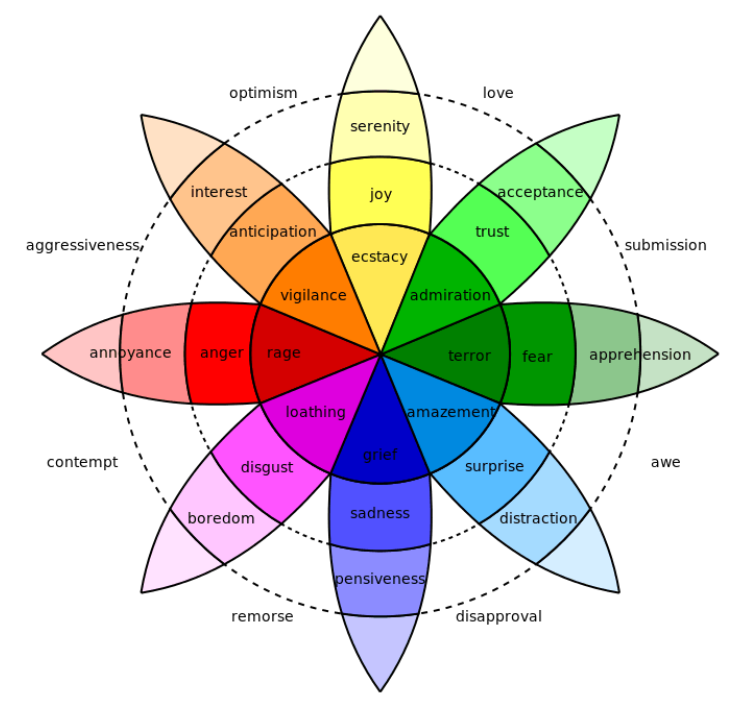
\includegraphics[width=0.5\textwidth]{./img/nlp/emozioni.png}
            \caption{Classificazione delle emozioni}
            \label{fig:emozioni}
      \end{figure}
\end{definizione}
\subsection{Rappresentazione del testo}
Il primo passo consiste nel capire come rappresentare il testo. Questo passaggio
è necessario per passare da una misura qualitativa a una misura quantitativa.

Una prima soluzione è quella di rappresentare il testo tramite un dizionario
di parole. Questo metodo è molto semplice e permette di rappresentare il testo
come un vettore di bit, dove il bit $i$-esimo è a $1$ se la parola $i$-esima
è presente nella frase. Questo metodo però ha dei problemi:
\begin{itemize}
      \item Il vettore che rappresenta la frase è molto grande e sparso.
      \item Perdiamo l'ordinamento delle parole.
\end{itemize}
Un ulteriore metodo consiste nella \textbf{BagOfWord}, ovvero si rappresenta una
frase tramite un vettore in uno spazio. Il problema di questo approccio è legato
al fatto che manca la composizionalità delle parole.

Possiamo usare una rappresentazione deep basata su \textbf{word2vec}, essa consiste
nello scrivere la parola sulla base dei termini che lo precedono e che lo seguono.
Si ha quindi una strategia simile alla BagOfWord, ma mantenendo la composizionalità.

Word2Vec è un modello che viene usato per creare una rappresentazione vettoriale
delle parole. Esistono due tipologie di Word2Vec:
\begin{itemize}
      \item \textbf{skip-gram}: partendo da una parola del documento cerco di
            predire l'intorno di essa.

            Per ottenere questo risultato, la parola viene codificata attraverso
            \textbf{one-hot-vector}, ovvero un bitvector lungo quanto il
            vocabolario, con un bit a $1$ nella posizione associata alla parola.

            Successivamente si costruisce una rete neurale tipo Encoder-Decoder
            che preso in input il bitvector, fornisce in output un vettore
            lungo tanto quanto il vocabolario con una probabilità associata ad
            ogni parola. La rappresentazione vettoriale coincide con quello che
            si ha nell'hidden layer, quindi la sua dimensione è decisa in fase di
            costruzione della rete.

            Il documento viene rappresentato dal vettore media dei vettori dei
            termini presenti nel documento.

            A differenza dalle rappresentazioni viste in precedenza, abbiamo un
            vettore di dimensione $n$ selezionato dalla rete. Il problema è che
            non andiamo a considerare il contesto del mondo.

            Esistono metodi più efficaci per rappresentare il testo come
            \textbf{USE} e \textbf{BERT}.
      \item \textbf{CBOW}: cerca di predire la parola sulla base del suo intorno.
\end{itemize}
Questi permettono di avere parole con lo stesso significato o simili vicine nello
spazio vettoriale. Inoltre, con questo approccio risulta possibile rappresentare
l'intero documento con un vettore ottenuto come media dei vettori delle parole
presenti in esso.

Una volta risolto il problema della rappresentazione si può passare alla fase
di classificazione. Questa può essere fatta in diversi modi:
\begin{itemize}
      \item \textbf{Lexicon-based}: si basa su un dizionario di parole associate
            a delle emozioni. Si contano le parole associate alle emozioni e si
            restituisce l'emozione con il conteggio maggiore. Se le emozioni hanno
            lo stesso numero di parole allora la frase è neutra.
      \item \textbf{Machine Learning}: si basa su un modello di classificazione
            che prende in input il vettore che rappresenta la frase e restituisce
            l'emozione.
\end{itemize}
\begin{nota}
      Nel primo caso risulta importate scegliere bene il lessico, perché le parole
      possono essere positive o negative in base al contesto.
\end{nota}
\section{Semantic Ambiguity}
Uno dei tanti problemi che si riscontrano nell'analisi del linguaggio naturale
è l'ambiguità delle parole. Questo è molto importante, in quanto per comprendere
un testo bisogna capire a che cosa ogni token si riferisce.

I problemi che si possono riscontrare nel riconoscimento dei token sono riportati
di seguito:
\begin{enumerate}
      \item Il linguaggio con cui è scritto il testo è \textbf{rumoroso}, ovvero
            sono presenti errori ortografici, ambiguità e polisemia (a una parola
            posso associare più significati).
      \item \textbf{Out of vocabulary} (OOV): quando il modello non ha mai
            incontrato delle parole che gli vengono fornite come input. Ad esempio,
            se in fase di training il modello ha appreso la frase ``The Big Bang
            Theory'', mentre in fase di test gli viene fornita la frase ``TBBT'',
            il modello non riconoscerà la parola.
      \item \textbf{Out of Knowledge base}: quando il modello non ha una
            rappresentazione dell'entità nella base di conoscenza. Ad esempio,
            il nome di un nuovo prodotto.
\end{enumerate}
\subsection{Name entity recognition}
\begin{definizione}[\textbf{Named Entity Recognition}]
      La \textbf{Named Entity Recognition} (NER) è una tecnica che permette di
      identificare le entità all'interno di un testo e classificarle in categorie
      predefinite.
\end{definizione}
\begin{definizione}[\textbf{Surface Form}]
      La \textbf{Surface Form} è la rappresentazione di un'entità indipendente
      dalla semantica nella frase.
\end{definizione}
Per svolgere questo task si utilizzano dei modelli neurali i quali escono dalla
classica idea di machine learning, in quanto l'output non è più un singolo valore
ma una sequenza di valori. Questo problema viene risolto con i modelli \textbf{sequence
      prediction}.

Nel nostro caso si ha una sequenza di osservazioni e si impara per prevedere la
sequenza ottimale di etichette che devono essere associate alle osservazioni.
In questo modo si considera nella predizione il contesto delle osservazioni
facenti parte della sequenza, quindi non si effettua il training sulle singole parole.
\subsubsection{Conditional Random Fields}
Il modello che viene utilizzato per risolvere il problema di NER è il \textbf{Conditional
      Random Fields} (CRF). Questo modello è un modello grafico probabilistico che
massimizza la probabilità condizionata delle etichette della sequenza di input.

Questo modello può essere come un grafo dove si hanno dei nodi che rappresentano
le osservazioni e degli archi che rappresentano le dipendenze tra le etichette.

Le parole sono connesse solamente alle etichette, mentre è presente una relazione
temporale tra le etichette. Questo modello è un modello di Markov del primo ordine,
in quanto si considera solamente la parola precedente.

Vediamo ora un esempio di struttura di un CRF:
\begin{figure}[!ht]
      \centering
      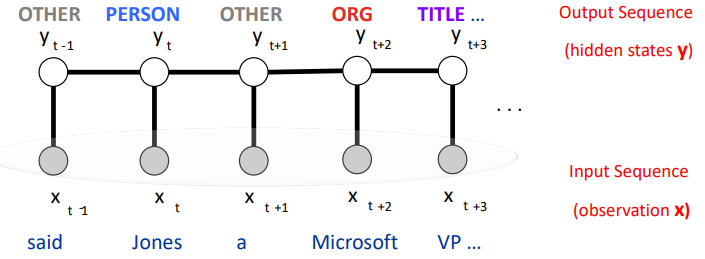
\includegraphics[width=0.5\textwidth]{./img/nlp/crf.png}
      \caption{Struttura di un CRF}
      \label{fig:crf}
\end{figure}

In fase di training si impara $P(y|x)$, dove $y$ è il vettore delle etichette
mentre $x$ è il vettore delle parole.
\begin{equation}
      P(y|x) = \frac{1}{Z_x} \prod_t \phi(y_t,y_{t-1},x ,t)
\end{equation}
dove $\frac{1}{Z_x}$ rappresenta una costante di normalizzazione, mentre la
funzione $\phi(y_t,y_{t-1},x ,t)$ può essere scritta come:
\begin{equation}
      \phi(y_t,y_{t-1},x ,t) = \exp (\sum_k\lambda_k f_k(y_t,y_{t-1},x,t))
\end{equation}
dove $f_k(y_t,y_{t-1},x,t)$ sono delle \textbf{feature function}, ovvero delle
funzioni predeterminate che valutano diverse proprietà in base all'osservazione e
all'etichetta precedente al tempo $t$. È importante che queste funzioni abbiano
almeno due stati di uscita, possiamo considerare le feature function come degli
\textbf{if}.

Le feature function possono essere di due tipologie:
\begin{itemize}
      \item \textbf{State} $f_i(y_t, x) \in \mathbb{R}$: valutano lo stato in
            cui ci si trova in quel tempo. Nello specifico valutano la relazione
            che c'è tra la parola $x_t$ e la sua etichetta $y_t$.
      \item \textbf{Transition} $g_i(y_t, y_{t - 1}, x) \in \mathbb{R}$: modellano
            la dinamica dell'etichettatura. Misurano la relazione tra l'etichetta
            della parola al tempo $t$ e l'etichetta della parola al tempo $t - 1$.
            Le definisco a runtime perché si applicano alle etichette.
\end{itemize}

Quanto ottenuto è un modello log-lineare, quindi, possiamo riscrivere il calcolo
della probabilità condizionata come:
\begin{equation}
      P(y|x) = \frac{\exp \sum_{t = 1}^T\left( \sum_i \lambda_i f_i(y_t,x) +
      \sum_j \mu_j g_j(y_t,y_{t-1},x) \right)}{Z_x}
\end{equation}
Dato che le funzioni sono note, dobbiamo imparare i parametri $\lambda_i, \mu_j$,
per fare questo, si massimizza la \textbf{log-likelihood} del modello rispetto
alle osservazioni, ovvero:
\begin{equation}
      L_{\lambda,\mu} = \sum_{t} \log P(y_t|x_t, \lambda, \mu) = \sum_k \left[
            (\lambda, \mu) \cdot F(y_k, x_k) - \log Z_{\lambda, \mu}(x_k) \right]
\end{equation}
L'inferenza consiste nel determinare la migliore sequenza di etichette data una
sequenza di osservazioni.

Il processo di inferenza avviene tramite l'algoritmo di \textbf{Viterbi}, il quale
trova la sequenza di etichette che massimizza la probabilità condizionata. Si ha
una struttura simile a una rete neurale, dove ogni layer è composto da tanti nodi
quante le etichette possibili. La rete e fully connected e ogni arco ha un peso
associato, determinato dalla feature function.

La valutazione del modello si effettua in due metodologie:
\begin{itemize}
      \item \textbf{Exact Match}: considero corretta la predizione se tutta l'entità
            viene riconosciuta correttamente. Utile se devo fare sentiment analysis.
      \item \textbf{Partial Match}: considero corretta la predizione se l'entità
            viene riconosciuta parzialmente. Utile se devo fare retrival del db.
\end{itemize}
\subsection{Named Entity Linking}
Una volta riconosciuta l'entità spesso si effettua \textbf{named-entity linking},
ovvero partendo dalla surface form si cerca di associare l'entità ad una risorsa
presente nella base di conoscenza.

Questo task viene svolto nel seguente modo:
\begin{enumerate}
      \item Si cerca nella base di conoscenza il token usando la sua surface form.
      \item Si prendono i primi $k$ risultati e si calcola la similarità tra
            la surface form e il risultato. Questo può essere fatto tramite
            diverse metriche e considerando diversi attributi.
      \item Si restituisce l'entità con la similarità maggiore.
\end{enumerate}

Un esempio di pipeline per il name entity linking è riportato di seguito:
\begin{figure}[!ht]
      \centering
      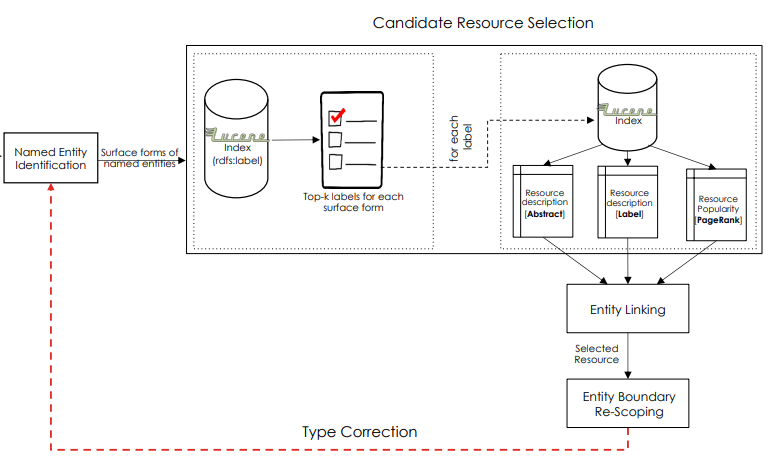
\includegraphics[width=0.5\textwidth]{./img/nlp/nel.png}
      \caption{Pipeline per il Named Entity Linking}
      \label{fig:nel}
\end{figure}

Un possibile approccio è quello di utilizzare il \textbf{candidate resource selection},
nel quale per ogni per ogni entità $e_j$ si calcola il suo score nella base di conoscenza
con riferimento alla risorsa $c_k$.
\begin{equation}
      KB(e_j, c_k) = \alpha \cdot \texttt{lex}(e_j, l_{c_k}) + (1 - \alpha) \cdot \texttt{cov}(e_j, c_k)
\end{equation}
dove:
\begin{itemize}
      \item $\texttt{lex}(e_j, l_{c_k})$ è la similarità lessicale tra l'entità
            $e_j$ e la label associata alla risorsa $c_k$ candidata.
      \item $\texttt{cov}(e_j, c_k)$ è la covarege basata sulla coerenza che l'entità
            rispetto alla base di conoscenza e alla popolarità della risorsa candidata $c_k$.
\end{itemize}
A questo punto si seleziona la risorsa con il punteggio maggiore e si restituisce
l'entità associata.
\subsection{Word sense disambiguation}
Si cerca di comprendere il significato della parola che è accettato comunemente.
Questo ci permette di disambiguare il significato della parola dal punto di
vista del senso. Dobbiamo però considerare che il significato della parola può
dipendere da quello che la circonda.

Gli approcci che possono essere utilizzati per risolvere questo problema sono:
\begin{itemize}
      \item \textbf{Knowledge-based Disambiguation}: sono sistemi basati su basi
            di conoscenza, come dizionari e tesauri.
      \item \textbf{Supervised Disambiguation}: sono sistemi che richiedono dati
            etichettati per funzionare.
      \item \textbf{Unsupervised Disambiguation}: sono sistemi che non richiedono
            dati etichettati per funzionare.
\end{itemize}
\subsubsection{Knowledge-based Disambiguation}
Nei metodi basati su basi di conoscenza, la disambiguazione della parola si
effettua tramite un dizionario machine readable e dati raw. Non servono quindi
dei dati etichettati e si lavora su parole appartenenti alle open class.

Nei dizionari si possono trovare molte informazioni utili per la disambiguazione,
possiamo trovare i sinonimi, le definizioni, le relazioni tra le parole, etc.

Un primo algoritmo è \textbf{Lesk algorithm}, definisce il senso delle parole
nel contesto confrontando le definizioni si sovrapposizioni. Il funzionamento di
questo algoritmo è il seguente:
\begin{itemize}
      \item Prende dai machine readable dictionary le definizioni di tutte le
            parole che si vogliono disambiguare.
      \item Determina gli overlap tra tutte le coppie di parole da disambiguare.
      \item Seleziona il significato in base al massimo numero di overlap.
\end{itemize}
Questo algoritmo è molto pesante dal punto di vista computazionale in quanto
si devono calcolare tutte le combinazioni di parole.

Per questo motivo, è stata introdotta una variante detta \textbf{Simplified Lesk}
il quale funziona nel seguente modo:
\begin{itemize}
      \item Prende dai machine readable dictionary le definizioni della parola
            che si vuole disambiguare.
      \item Calcola l'overlap tra la parola da disambiguare e tutte le altre
            della frase.
      \item Seleziona il significato con il massimo overlap.
\end{itemize}
\subsubsection{Unsupervised Disambiguation}
Questi approcci tentano di rimuovere il collo di bottiglia legato alla necessità
di avere una base di conoscenza. Infatti, non si ha la necessità di avere una
base di conoscenza o etichette, ma il senso viene definito dal contesto.

Un esempio di algoritmo unsupervised è \textbf{Word Sense Induction} oppure
\textbf{Word Sense Disambiguation}.

L'algoritmo \textbf{Chinese Whispers} è un algoritmo di clustering che si basa
su grafi non orientati e senza pesi sugli archi. Questo algoritmo funziona nel
seguente modo:
\begin{itemize}
      \item Inizialmente, ogni nodo è assegnato a una classe.
      \item In modo iterativo, si seleziona un nodo in modo casuale e lo si assegna
            alla classe con la quale il nodo ha più connessioni. In caso di
            parità, si assegna il nodo a una classe casuale.
\end{itemize}
I vantaggi di questo algoritmo sono legati all'efficienza e al fatto che non è
necessario specificare nessun parametro. Tuttavia, il principale svantaggio è
che non è deterministico e ci sono situazioni in cui non converge.

Un altro modo è quello di utilizzare un approccio basato sui grafi. In questo caso
si parte da una fase di preprocessing del testo, dove si eliminano le stop-words
e si effettua il part-of-speech tagging. Successivamente si costruisce un grafo
dove i nodi sono le parole e gli archi sono le relazioni tra le parole. Infine,
si pesano gli archi in base alle co-occorrenze delle parole.

Una volta costruito il grafo, si applica l'algoritmo di clustering per trovare
i cluster di parole. 
\section{Topic Models}
\begin{definizione}
      Il \textbf{topic recognition} è il problema di riconoscere il tema data una
      collezione di documenti.
\end{definizione}

Il riconoscimento è costruito sulla ricerca di pattern sintattici di parole collegate
da un topic comune, si basa sull'idea che il topic dipende dall'insieme di parole
che compaiono con frequenza maggiore. Di conseguenza è un processo non supervisionato.

Alla fine, data una collezione di documenti, si assume che per ogni documento ci
siano diversi topics, ottenendo quindi una una distribuzione di topic per ognuno
di essi. Ogni topic può essere visto, a sua volta, come una distribuzione di parole
all'interno del documento. Quindi noi \textbf{osserviamo} i documenti e le parole
dai quali si devono predire i topic \ref{fig:topic}.
\begin{figure}[!ht]
      \centering
      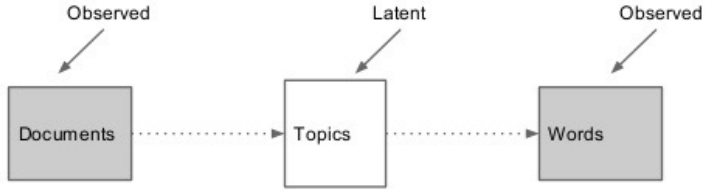
\includegraphics[width=0.7\textwidth]{img/nlp/topic_model.png}
      \caption{Rappresentazione dei topic}
      \label{fig:topic}
\end{figure}
\begin{nota}
      I topic li possiamo vedere come delle word-cloud e le etichette dei topic
      possono essere identificate da un umano o automaticamente.
\end{nota}
Una generica pipeline sul topic modelling consiste nel prendere delle collezioni
di documenti ed eseguire su di esse dei topic model. Questi permettono di
estrarre dalla collezione di documenti:
\begin{itemize}
      \item I topic, ovvero cluster di parole.
      \item Distribuzione dei topic in ciascun documento.
      \item Distribuzione delle parole nei topic.
\end{itemize}

Più precisamente la modellazione dei topic si basa sui seguenti concetti:
\begin{itemize}
      \item \textbf{Ogni documento è un insieme di topic}. Specifica che ogni
            documento può essere definito da una distribuzione di topic.
      \item \textbf{Ogni topic è un mix di parole}. Specifica che ogni topic ha
            una distribuzione delle parole che ne descrivono il contenuto.
\end{itemize}
Gli strumenti che si utilizzano per risolvere il seguente problema sono:
\begin{itemize}
      \item \textbf{Frequentisti} o \textbf{Statistical based}: unigramma, mixture
            of unigramm, latente dirichlet allocation. Per queste tipologie, le
            metriche di valutazione sono PMI, RBO e KL.
      \item \textbf{Neural based}: contextualized topic model, neural-based. Vengono
            valutati usando la metrica WED.
\end{itemize}

I modelli neurali permettono di trovare delle differenze semantiche rispetto al
contesto, cosa che non fanno i modelli frequentisti.
\subsection{Unigram model}
Questo modello si basa sull'assunzione che esista un solo topic nella collezione.
Essendoci un solo topic allora il compito diventa stimare la distribuzione delle
parole del dizionario rispetto al topic ($p(w)$).

Quindi data una parola del dizionario, questa può essere osservata se presente
in un documento oppure non osservata se non è presente della collezione.
Per ogni parola possiamo calcolare la distribuzione rispetto ai documenti,
ovvero la probabilità di presenza della parola nei vari documenti, oppure possiamo
calcolare per ogni documento la distribuzione delle parole.
\begin{equation}
      p(\vec{w}) = \prod_{n = 1}^{N} p(w_n)
\end{equation}
\begin{figure}[!ht]
      \centering
      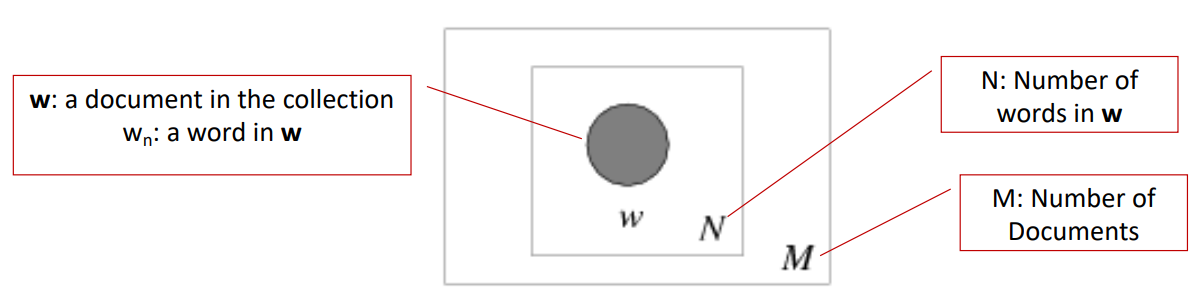
\includegraphics[width=0.5\textwidth]{./img/nlp/unigram.png}
      \caption{Unigram model}
      \label{fig:unigram}
\end{figure}
\subsection{Mixutere Unigram model}
Simile all'\textit{Unigram model} con la differenza che si assume di avere più
topic nella collezione, i quali sono noti, ma con un solo topic per documento.

Quindi per ogni parola possiamo calcolare la sua distribuzione rispetto ai topic,
e per ogni topic possiamo calcolare la distribuzione dei documenti. Questo ci
permette di avere per ogni parola abbiamo una distribuzione di topic e per ogni
documento abbiamo una distribuzione di topic. In formule:
\begin{equation}
      p(\vec{w}) = \sum_z p(z) \prod_{n = 1}^{N} p(w_n|z)
\end{equation}
dove $z$ è il topic e $w_n$ è la parola nel documento $\vec{w}$.
\begin{figure}[!ht]
      \centering
      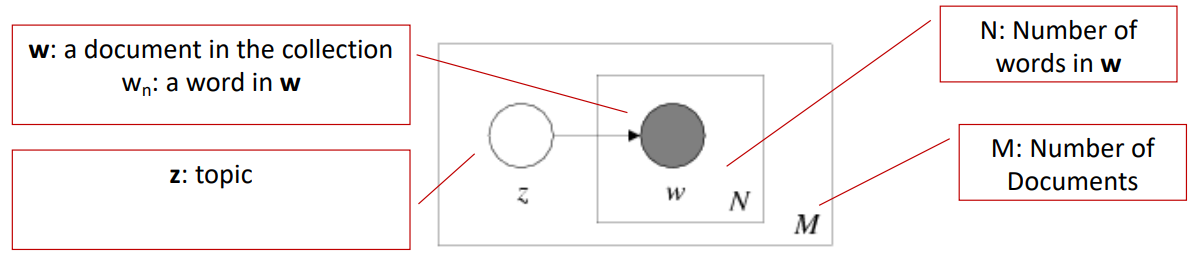
\includegraphics[width=0.5\textwidth]{./img/nlp/mixture.png}
      \caption{Mixture Unigram model}
      \label{fig:mixture_unigram}
\end{figure}
\begin{nota}
      In questo modello il numero dei topic deve essere dato.
\end{nota}
\subsection{Latent Dirichlet Allocation}
Questo modello si basa sulla teoria bayesiana dove nulla è fissato e tutto è
campionabile. La principale assunzione è che ogni documento è costituito da più
topic e che:
\begin{itemize}
      \item Ogni topic è una distribuzione su più parole.
      \item Ogni documento è un insieme di topic.
      \item Ogni parola è all'interno di un topic.
\end{itemize}
LDA si basa su due processi:
\begin{itemize}
      \item \textbf{Generative process}: processo che genera i documenti partendo
            da delle distribuzioni note.
      \item \textbf{Inferential process}: processo che permette di inferire i topic
            osservando le parole nei documenti.
\end{itemize}
Partendo dal fatto che un \textit{topic} è una distribuzione di parole di un
vocabolario $W$, il quale consiste di $N$ parole univoche che rappresentano il
documento, possiamo definire una \textbf{word topic distribution}, ovvero:
\begin{equation}
      P(w|z)
\end{equation}
la quale rappresenta la probabilità di una parola del vocabolario ($w$) all'interno
di un topic ($z$). Il processo di costruzione di questa distribuzione parte da
una versione randomica, la quale viene migliorata in modo iterativo con un
funzionamento simile a quello visto per Markov Chain Monte Carlo.

Oltre a questa, ad ogni documento è associata una \textbf{document topic distribution},
ovvero:
\begin{equation}
      P(z|d)
\end{equation}
la quale rappresenta la probabilità di osservare un topic ($z$) all'interno di
un documento ($d$). Anche questa distribuzione, come la precedente, viene costruita
in modo iterativo partendo da una versione randomica.

Dato un topic model LDA, il quale consiste nelle probabilità $P(w|z)$ e $P(z|d)$,
un documento $d$ è composto da $n$ parole non univoche ed è generato secondo il
seguente processo generativo:
\begin{itemize}
      \item Per ogni parola $w$ del documento $d$:
            \begin{itemize}
                  \item Campiona un topic $z$ da $P(z|d)$.
                  \item Campiona una parola $w$ da $P(w|z)$.
            \end{itemize}
      \item Aggiungi la parola $w$ al documento $d$.
\end{itemize}

Il precedente processo può essere rappresentato con il diagramma riportato in
figura \ref{fig:lda}.
\begin{figure}[!ht]
      \centering
      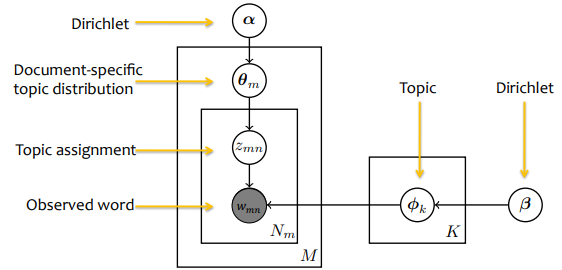
\includegraphics[width=0.5\textwidth]{./img/nlp/lda.png}
      \caption{Diagramma di LDA}
      \label{fig:lda}
\end{figure}

In questo diagramma abbiamo la \textbf{Dirichlet prior} $\alpha$ applicata alla
document topic distribution e la \textbf{Dirichlet prior} $\beta$ applicata alla
word topic distribution.

Il termine $\alpha$ è un iperparametro che permette di stabilire la probabilità
a priori che il topic sia presente nel documento. Se $\alpha$ è alto, allora mi
aspetto che ci siano tanti topic nel documento, mentre se è basso mi aspetto che
ci sia un topic dominante nel documento.

Il termine $\beta$ è un iperparametro che permette di stabilire la probabilità
a priori che la parola sia presente nel topic. Se $\beta$ è alto, allora mi aspetto
che ci siano molte parole nel topic, mentre se è basso mi aspetto che ci siano
poche parole nel topic.

$\alpha, \beta$ sono iperparametri che danno la distribuzione a priori poi effettuo
il train per aggiustare meglio $\theta$ e $\phi$.

Il processo di \textbf{inferenza} è strutturato nel seguente modo:
\begin{enumerate}
      \item \textbf{Inizializzazione}: vengono assegnati i topic in modo randomico
            ad ogni parola del documento. Questo permette di stabilire le
            frequenze semplicemente contando le parole.
      \item \textbf{Aggiornamento}: per ogni parola di un documento, si aggiorna
            il topic assegnato usando le frequenze di tutte le parole tra word e
            topic in aggiunta a una variabilità dalla distribuzione di Dirichlet.
            Questo processo prende il nome di \textbf{Collapsed Gibbs Sampling}.
      \item \textbf{Ripeto}: l'aggiornamento del punto precedente viene ripetuto
            per tutte le parole di tutti i documenti.
      \item \textbf{Iterate}: si ripete tutto il processo per un numero di iterazioni
            fissato.
\end{enumerate}

La fase di aggiornamento avviene tramite il \textbf{Collapsed Gibbs Sampling}:
\begin{equation}
      p(z_t = j | z_t, w_t,d_t) = \frac{C_{w, j}^{WT} + \beta}{\sum_{w = 1}^{W} C_{w, j}^{WT} + W\beta}
      \frac{C_{d, t}^{DT} + \beta}{\sum_{t = 1}^{T} C_{d, t}^{DT} + T\alpha}
\end{equation}
dove:
\begin{itemize}
      \item $p(z_t = j | z_t, w_t,d_t)$ è la probabilità di avere il topic $j$
            per la parola $w_t$ nel documento $d_t$.
      \item $\frac{C_{w, j}^{WT} + \beta}{\sum_{w = 1}^{W} C_{w, j}^{WT} + W\beta}$
            è la probabilità di avere la parola $w$ nel topic $t$. In pratica la
            formula mette a numeratore il numero di volte che la parola $w$ appare
            nel topic $t$. Mentre a denominatore si ha la somma delle parole nel
            topic $t$ più il numero di parole nel vocabolario.
      \item $\frac{C_{d, t}^{DT} + \beta}{\sum_{t = 1}^{T} C_{d, t}^{DT} + T\alpha}$
            è la probabilità di avere il topic $t$ nel documento $d$. In pratica
            la formula mette a numeratore il numero di volte che il topic $t$ appare
            nel documento $d$. Mentre a denominatore si ha la somma dei topic
            nel documento $d$ più il numero di word.
\end{itemize}
\subsection{Valutazione dei Topic model}
Per valutare i modelli precedentemente introdotti possiamo usare delle misure
basate su \textit{Shared Word Tokens}:
\begin{itemize}
      \item \textbf{Topic Coherence}: Average Pointwise Mutual Information (PMI)
            tra le parole del topic.
            \begin{equation*}
                  PMI(t_i, t_j) = \frac{1}{t^2} \sum_{u \in t_i} \sum_{v \in t_j} PMI(u, v)
            \end{equation*}
            dove $t$ è il numero di parole per ogni topic.
      \item \textbf{Topic diversity}: Rank-Biased Overlap (RBO), considera l'overlap
            delle liste di parole in base alla scala.
            \begin{equation*}
                  RBO(S, T, p) = (1 - p) \sum_{k = 1}^{\infty} p^{k - 1} A_k
            \end{equation*}
\end{itemize}
Una diversa metrica di confronto, che si basa sulla distribuzione di probabilità
dei topic, è la \textbf{Kullback-Leibler divergence} (KL):
\begin{equation}
      KL(p||q) = \sum_{i} p(i) \log \frac{p(i)}{q(i)}
\end{equation}
\begin{nota}
      Questa metrica è asimmetrica, ovvero l'ordine con cui confronto le distribuzioni
      è importante.
\end{nota}
Solitamente si confronta la distribuzione con distribuzioni note, come ad esempio
la distribuzione uniforme, la Junk Topic Distribution, etc.
